\section{Casi d'uso}
\subsection{Introduzione}
In questa sezione vengono descritti i casi d'uso individuati dal gruppo \gruppo{}.
I casi d'uso analizzati fanno riferimento a tutte le funzionalità che il software di sincronizzazione dovrà fornire all'utente finale.

\subsection{Attori}


\subsection{UC1 - Autenticazione}
\begin{figure}[H]
    \centering
    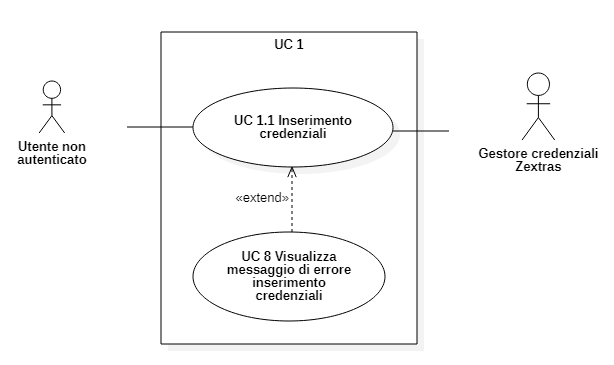
\includegraphics[scale = 0.7]{components/img/UC1.png}
    \caption{UC1 - Autenticazione}
\end{figure}
\begin{itemize}
\item \textbf{Attore Primario:} Utente;
\item \textbf{Precondizione:} L'utente non è autenticato all'interno dell'applicazione;
\item \textbf{Postcondizione:} L'utente ha effettuato il login usando le credenziali di Zextras Drive;
\item \textbf{Scenario principale:}
    \begin{enumerate}
    \item L'utente avvia l'applicazione per la prima volta;
    \item L'utente inserisce le credenziali Zextras Drive;
    \end{enumerate}
\item \textbf{Estensioni:}
\begin{itemize}
\item L'utente inserisce delle credenziali che non sono valide;
\item L'utente è offline e non è possibile contattare il Gestore credenziali di Zextras.
\end{itemize}
\end{itemize}